
%\newcommand{\state}{\mathbf{s}}
%t
%\newcommand{\command}{\mathbf{u}}
%\newcommand{\conf}{\mathbf{J}^{\eeposition}}
%\newcommand{\eeJacDot}{\mathbf{\dot{J}}^{\eeposition}}
\chapter{MPC-based Constraints Compatibility for Whole-Body QP Control}\label{chap:mpc ref gov}

%Constraints compatibility~\cite{decre2009icra,rubrecht2010iros,delprete2018ral,meguenani2017phdThesis}
%TODO \cite{tan2015robio} MPC to predict the object motion, with which the robot must avoid collision, while minimizing the robot joint torque jump. The predicted distance is forwarded to reactive QP to be considered in the collision constraint formulation. The task trajectory is not modified.
% \begin{itemize}
% %	\item The posture task is no longer a regularization task intended mainly to solve the remaining redundancies, it brings an interesting behavior for the reactive whole-body QP. Namely, our formulation enables a planning in both task-space and joint-space.
% %	\item Increase posture task gains
% %	\item Remove dynamic constraints 
%% 	\item Consider other constraints that are potentially in conflict, e.g., a collision avoidance and CoM constraints. Namely, if you avoid the collision you may violate the CoM constraint
% %	\item Consider HRP-4 ({\color{red} issue with the floating-base orientation})
% %	\item Consider Niels random target generator
% %	\item Imagine MPC-based adaptive gains  
% %	\item Discrete-time CBF for MPC
% \end{itemize}

In the previous chapter, we proposed a robust feedback closed-loop QP control formulation in the case of kinematic-controlled robots. Task and set robust stability have been formally proved and validated in real experiments. In particular, the kinematic constraints, formulated in terms of $\genActConfDDot$, are introduced to QP online in the vicinity of the boundary. %In the case of multi-objective control, robust stability of relaxed tasks has also been proved. 
%In the previous chapter, we proposed a novel approach to unify observation and control tasks by formulating them as coupled control objectives via task-space QP control paradigm. In particular, we explained how this approach fits nicely with the human-robot handover application where the results shows great adaptability to the human intention w.r.t the HOL and object configuration. 

So far, state-of-the-art prioritized multi-objective QP approaches focused on smooth online tasks introduction, removing or priority swapping to lower the subsequent discontinuity that may occur at the joint-acceleration and torque. On the other hand, the constraints have a higher priority over the tasks. The latter are generally achieved ‘at best’ while fulfilling all the constraints. Unfortunately, introducing constraints online may make the QP infeasible (as explained in \cref{subsec-chap0:kinematic constraints formulation} and exemplified in \cref{fig:configs}). In fact, all the constraints have the same level of priority. Consequently, if at least two constraints conflict, the constraint-set becomes empty. We say then that these constraints are incompatible~\cite{decre2009icra,rubrecht2010iros,delprete2018ral,meguenani2017phdThesis}. This situation is typically exemplified by the collision avoidance constraint formulated as in  \cref{chap:adaptive gains} and the hardware limitations.
 %As seen in \cref{chap:adaptive gains}, the former imposes a boundary on the necessary joint acceleration to apply until reaching the boundary with zero velocity, whereas the latter specifies the set of affordable amount of joint acceleration. 
If the collision avoidance constraint requires joint acceleration amplitudes higher than what is affordable by the hardware limitations, then the QP fails to find a solution that satisfies both constraints (\cref{fig:configs}\subref{subfig:config3}).  This is expected as the collision-avoidance constraint formulation does not account for the hardware limitations.~\cite{ames2021csl} proposed a holistic CBF formulation to avoid collisions while incorporating the control input bounds. However, the latter are considered constant, and the approach has been validated on a low dimension toy-example only. More importantly, even if the hardware limitations are ignored from the QP constraint set to avoid infeasibility, the actuators cannot effectively apply the desired joint acceleration and the robot finishes by colliding with the object in question.   

The main reason for this infeasibility is the Whole-Body QP (WBQP)\footnote{In this chapter, the ‘whole-body’ term is used to emphasize the distinction with the QP used for MPC formulation. } myopia. Being purely reactive, the WBQP controller solves the optimization problem based on the current robot state. However, dealing with potential incompatible  constraints requires a prediction of the future robot states  to know what are the current actions to do to ensure the viability of the control problem in the next iterations. 
%Nevertheless, all the constraints have the same level of priority. Consequently, if at least two constraints are in conflict, the QP will fail to find a feasible solution. Hence, online 
  
Since the robot motion is essentially driven by the tasks' dynamics defined in QP, our idea is to ensure the constraints compatibility at the task level by modifying task targets to account for the hardware limitations and collision constraints. For instance,  instead of arbitrarily defining set-point or trajectory references and let the QP constraints take care of avoiding collisions at the risk of running into infeasibility, we compute a sequence of \emph{optimal} targets that converge to the reference targets while satisfying the hardware limits and avoiding collision if any (\cref{fig:QPvsMPC-QP}). These optimal targets are computed by the so-called reference governor (see~\cite{bemporad1998tac}, and also a recent survey in~\cite{garone2017automatica}.
%to computed tasks targets such that the robot constraints are accounted for. Namely, instead of arbitrarily defining  set-point or  trajectory references and let the reactive QP ensure  potential collision avoidance and hardware limits, we compute optimal targets that converge to the reference targets while accounting for the QP constraints. 
In this chapter, we propose to formulate such a reference governor using a linear MPC layer on top of the closed-loop system constituted by the WBQP controller and the robot. Based on the system's closed-loop dynamics, the MPC  predicts the robot state over a finite horizon and enforces the different constraints on these predicted states. Hence, MPC outputs \emph{constraints-compatible} optimal targets to be tracked by the WBQP tasks. In \cref{sec-chap5:problem definition}, we expose the control problem. Then, we explicit the proposed closed-loop MPC-WBQP in \cref{sec-chap5:MPC-QP} where we derive the MPC dynamic model and explicit the MPC implementation. In \cref{sec-chap5:experiments}, we validate the proposed approach in simulation.
%, and to which the constraints fulfillment is delegated.  
%MPC accounts for the hardware limitations, joint-position and velocity constraints as well as other safety constraints expressed in terms of distance (e.g., collision avoidance, CoM, etc.). Instead of finding the right time when to trigger the deceleration in QP, MPC will then output optimal targets to be tracked by the QP tasks such that the above constraints fulfilled.
%By predicting over a preview horizon the robot state governed by the tasks dynamics, MPC governs the QP 

%enforces will then output optimal targets to be tracked by the QP tasks such that the  that deviate from the reference trajectories if the predicted robot states get closer to a collision an obstacle. 
%\begin{figure}
%	\centering
%	\includegraphics[width=0.95\columnwidth]{convex-nonconvex sets}
%	\caption{Non-empty (left) and empty (right) QP feasibility domains in the case of a 2-DoF robot. The constraints are $\confDDot_{\min}\leq\confDDot\leq\confDDot_{\max}$ (rectangle) and an other constraint (e.g., collision avoidance constraint) in the form $\mathbf{A}\confDDot\leq \bm{b}$ defining a half-space ($\mathbf{A}\inR^{1\times n}$ is a row matrix).}
%	\label{fig:convex-nonconvex-sets}
%\end{figure}
\begin{figure}
	\centering
	\includegraphics[width=0.95\columnwidth]{QPvsMPC-QP}
	\caption{Classical approach (left): reference target beyond the obstacle, WBQP collision constraint takes care of avoiding the collision with the wall. Proposed approach (right): sequence of optimal targets (edge color gradually shifts from blue to pink according to the time evolution) are tracked by WBQP such that the collision with the wall is avoided. The red point denotes the initial task-space state.}
	\label{fig:QPvsMPC-QP}
\end{figure}
\section{Problem Definition}\label{sec-chap5:problem definition}
We here consider a fixed-base manipulator moving in free space without contacts (the notations in \cref{rem:fixed-base robot} are followed). The joint position, velocity and acceleration are denoted as $\conf,\confDot,\confDDot\inR^{n}$.
The multi-body robot dynamics writes
$\massMat(\conf) \confDDot + \nnLinTorqueMat(\conf,\confDot)\confDot + \gravity  = \Tau$.
Furthermore, mechatronic hardware limits are encoded as lower and upper bounds on joint accelerations
${\confDDot}_{\min} \leq \confDDot \leq {\confDDot}_{\max}$ and joint torques
${\Tau}_{\min} \leq \Tau \leq {\Tau}_{\max}$.
The kinematic mapping between the robot end-effector position and the joint-space is formulated as
\begin{align}
	\label{eq:forward kinematics}
	\eeposition &= f_{\eeposition}(\conf)\inR^{m}, \\	
	\label{eq:forward velcotiy}\eevelocity &= \eeJac \confDot\inR^{m}, \\
	\label{eq:forward accleration}\eeacceleration &= \eeJac \confDDot + \eeJacDot \confDot\inR^{m}.
\end{align}

Let the primary task-space objective given by reference end-effector position, velocity and acceleration targets $\eepositionRef(t),\eevelocityRef(t),\eeaccelerationRef(t)\inR^m$,
%$\DES{\eeposition}, \blue{\DES{\eevelocity}}, \blue{\DES{\eeacceleration}} \inR^{3}$
and reference joint-space positions, velocities and accelerations $\refConf(t),\refConfDot(t),\refConfDDot(t)\inR^n$. 
 Furthermore, the robot safety is handled by keeping its configuration inside a set $\setC$ defined as $\setC=\left\{\conf\inR^n:h(\conf)\geq0\right\}$ where $h(\conf)$ is barrier function denoting the distance to the boundary $h(\conf)=0$ and which has to remain positive. 
 %other constraints need to be considered to ensure the robot safety. These constraints are typically written as lower bound on distance  $h(\conf)\geq0$
Hereafter, we drop the potential dependencies on time and $\conf$ for ease of reading.
%The control problem is to track or reach these targets precisely and as fast as possible while respecting the hardware limits.

%Note that many planners proposed in literature operate either in joint-space only~\cite{berscheid2021arxiv} or in task-space only~\cite{}. %TODO add reference
%Here we are interested in a solution that performs planning in both spaces simultaneously similar to~\cite{lee2020cdc}, 
%however, satisfying realtime requirements.

%\section{Soft-Priority Multi-Objective QP}
Let us denote the constant user-defined proportional-derivative gains as diagonal matrices 
$\mathbf{P}_{\eeposition}, \mathbf{D}_{\eevelocity}\inR^{m\times m}$.
These allow formulating the task-space PD-feedback as
\begin{equation}
	\label{eq:taskspacePD}
	\PD{\eeacceleration} =  \eeaccelerationRef-\mathbf{P}_{\eeposition} ( \eeposition - \eepositionRef) 
	- \mathbf{D}_{\eevelocity} (  \eevelocity - \eevelocityRef) ,
\end{equation}
where the task-space references 
$\REF{\eeposition}, \REF{\eevelocity}, \REF{\eeacceleration}\inR^m$
are taken directly from a pre-planned trajectory or a static set-point target ($\REF{\eevelocity}= \REF{\eeacceleration}=\zeros$).
%TODO and  \red{\DES{\qaccelerations}} ?
For redundant robots, PD-feedback applies also in joint-space with diagonal matrices $\mathbf{P}_{\conf}, \mathbf{D}_{\confDot}\inR^{n\times n}$ to solve the remaining redundancies
\begin{equation}
	\label{eq:jointspacePD}
	\PD{\confDDot} =  \REF{\confDDot} - \mathbf{P}_{\conf} ({\conf}-\REF{\conf}) 	- \mathbf{D}_{\confDot} ( {\confDot}-\REF{\confDot} ) 	.
\end{equation}
To enforce the forward invariance and asymptotic stability of the set $\setC$, $\confDDot$ must remain in the set defined by the ECBF constraint as shown in \cref{chap:adaptive gains,chap:robust qp}
\begin{equation}\label{eq:ECBF constraint chap5}
	\ddot{h} + K_{\rm d}^{h} \dot{h} + K_{\rm s}^{h} h \geq0,
\end{equation}
with $\dot{h} = \actJacBfunc\confDot$, $ \ddot{h} = \actJacBfunc\confDDot+\actJacBfuncDot\confDot$ where $\actJacBfunc\inR^{1\times n}$ is the barrier function Jacobian.
%where $\REF{\conf},\REF{\confDot},\REF{\confDDot}\inR^n$ are joint-space references. 
%%\ak{where the desired joints come from?}
%
%TODO definejoint position, velocity and collision constraints.
In the context of multi-objective control, the two control objectives~\eqref{eq:taskspacePD} and~\eqref{eq:jointspacePD} are combined via a soft-hierarchy WBQP, which accounts for hardware limits and the robot safety
\begin{subequations}\label{eq:task&joint space QP with constraints}
	\begin{align}
		\underset{\confDDot}{\min} \ &\frac{\weight_{\eeacceleration}}{2}\norm{\eeJac \confDDot  - \left( \PD{\eeacceleration} - \eeJacDot \confDot \right)}^2  + \frac{\weight_{\confDDot}}{2}\norm{ \confDDot  -  \PD{\confDDot}}^2 \\
		\label{subeq:joint acc bounds}\text{s.t: }&{\confDDot}_{\min} \leq \confDDot \leq {\confDDot}_{\max} \\
		&\label{subeq:joint torque bounds}{\Tau}_{\min} - \nnLinTorqueMat\confDot - \gravity \leq \massMat\confDDot \leq {\Tau}_{\max}- \nnLinTorqueMat\confDot - \gravity \\ 
		& \label{subeq:safety constraint}\actJacBfunc\confDDot+\actJacBfuncDot\confDot + K_{\rm d}^{h} \dot{h} + K_{\rm s}^{h} h \geq0
	\end{align}
\end{subequations} 
where $\weight_{\eeacceleration},\weight_{\confDDot}>0$ are the control objectives' weights. 

Each of the constraints \cref{subeq:joint acc bounds,subeq:joint torque bounds,subeq:safety constraint} defines a set
	\begin{align}
		\label{eq:set acc bounds}{\cal F}_{\confDDot} &= \left\{\confDDot\inR^{n}:\cref{subeq:joint acc bounds}\right\}, \\ 
		\label{eq:set torque bounds}{\cal F}_{\Tau} &= \left\{\confDDot\inR^{n}:\cref{subeq:joint torque bounds}\right\}, \\ 
		\label{eq:set safety constraint}{\cal F}_{h} &= \left\{\confDDot\inR^{n}:\cref{subeq:safety constraint}\right\} .
	\end{align}
It is a common assumption to consider the   WBQP~\cref{eq:task&joint space QP with constraints} feasible~\cite{morris2013cdc,ames2017tac,ames2019ecc,ames2021csl}. That is to say, the feasibility domain ${\cal F}_{\rm QP}$ 
\begin{align}\label{eq:feasibility domain}
	{\cal F}_{\rm QP} = \begin{Bmatrix}
		\confDDot\inR^{n}: {\cal F}_{\confDDot} \cap {\cal F}_{\Tau} \cap {\cal F}_{h} 
	\end{Bmatrix} \neq \emptyset.
\end{align}
%Other safety aspects expressed as distance constraints $h(\conf)\geq0$ can be considered and expressed as shown in \cref{chap:adaptive gains}
%\begin{equation}
%	dsd
%\end{equation}

To ensure  safety while being  minimally invasive~\cite{tan2021tac}, ECBF constraint \cref{eq:ECBF constraint chap5} is typically inserted online in   WBQP if $h$ is sufficiently close to the boundary $h=0$. 
Nevertheless, the resulting ${\cal F}_{\rm QP}$ in \cref{eq:feasibility domain} is not guaranteed to be non-empty. In particular, if the necessary joint deceleration required by ${\cal F}_{h}$ to ensure safety cannot be allowed by the hardware limits, these constraints are incompatible, and QP fails to find a feasible solution (\cref{fig:configs}\subref{subfig:config3}).   

This limitation is due to the purely reactive nature of WBQP, which renders it \emph{myopic}: it does not predict the system trajectories, and thereby potential constraints conflict. Thus, the robot may run into non-desirable joint configurations, singularities, or even infeasibility due to incompatible constraints.
 
%Accurately predicting the evolution of the system would require updating 
% $\massMat, \nnLinTorqueMat$, $\bm{g}$, $\eeJac$ and $\eeJacDot$ according to the future states, which renders the problem non-linear.
%Recently,~\cite{kleff2021icra} proposed a realtime-capable non-linear MPC formulation for the torque joint-control of a robotic arm running at $1$~KHz. Nevertheless,
%their approach requires transforming the strict constraints into additional soft-objectives.
%Consequently, hardware limits cannot be guaranteed, and (hand-)tuning of weights becomes more critical. 

Hence, our approach consists of implementing a reference governor as an MPC layer on top of the reactive   WBQP controller~\eqref{eq:task&joint space QP with constraints} and to which we delegate the task of constraints compatibility by modifying, if necessary, the reference targets (\cref{fig:MPC-QP}). The MPC predicts the robot states and enforces the hardware limitations and safety constraints along the preview horizon. Then, it computes  a sequence of \emph{optimal} targets  $\eeposition^*,\eevelocity^*,\eeacceleration^*\inR^m$ and  $\conf^*,\confDot^*, \confDDot^*\inR^n$ forwarded to the   WBQP tasks~\cref{eq:taskspacePD,eq:jointspacePD}, respectively. By construction, the generated optimal target sequence converges toward the reference targets by following a path that is  \emph{constraints-compatible}, i.e., ensures both safety constraints and hardware limits. Our strategy consists then of removing ECBF constraint \cref{eq:ECBF constraint chap5} from WBQP and keeping only the hardware limits. 
Furthermore, MPC-WBQP enables a richer and more complex task-space robot motion compared to the straight-line-like motion obtained with the reactive  WBQP controller for set-point targets.

Note that our aim is not to supersede the  WBQP by MPC. Instead, the latter is implemented as an adds-on control scheme encapsulating the stable inner loop constituted by the robot and the  WBQP controller to mitigate the latter myopia. This architecture (similar to the one in~\cite{grandia2021icra,tan2015robio}) enables running the MPC at a lower frequency than the WBQP. Our approach is more generic than~\cite{tan2015robio} as the MPC directly modifies the reference targets, and it can encompass safe foot placement for quadruped locomotion as in~\cite{grandia2021icra}. Other approaches formulated whole-body  MPC controller, which renders the MPC computation-time critical w.r.t the real-time requirements. Safety-critical MPC has been proposed in~\cite{zeng2021acc2}. However, the approach has been validated in simulation for low-dimension racing cars collision avoidance. Recently,~\cite{kleff2021icra} proposed a real-time implementation of whole-body nonlinear MPC on 7-DoF robotic arm. However, the constraints are handled conservatively in the cost-function.     
%TODO \cite{tan2015robio} MPC to predict the object motion, with which the robot must avoid collision, while minimizing the robot joint torque jump. The predicted distance is forwarded to reactive QP to be considered in the collision constraint formulation. The task trajectory is not modified
% More importantly,  MPC layer mitigates mainly two issues thanks to its preview horizon: (i)  QP infeasibility when enforcing constraints especially when they are inserted  on-the-fly without accounting for the hardware limitation; (ii) handling the potential conflict between constraints (e.g., collision avoidance and CoM constraints) by finding task-space and joint-space targets that avoid or solve the potential conflict in the long run. 

In the next section, we detail our MPC implementation. First, we construct the model of the inner loop constituted by the WBQP controller and robot based on the closed-form solution of a weighted-prioritized  WBQP. After that, we define the MPC cost-functions and constraints.
%show how we formulate the MPC based on the QP controller formulation~\eqref{eq:task&joint space QP with constraints}.

\section{Task-space MPC with Soft-Hierarchy WBQP}\label{sec-chap5:MPC-QP}
The first step in formulating MPC is to have the dynamic model of the inner-loop to be controlled by MPC. Since the MPC computes optimal targets for the tasks, the inner-loop denotes the closed-loop formulation of the tasks combined in  WBQP. To do so, we need first to compute the closed-form solution of the   WBQP~\eqref{eq:task&joint space QP with constraints} in terms of $\confDDot$, which is then mapped to the task-space to have the corresponding closed-loop task dynamics. Nevertheless, the existence of inequality constraints in WBQP~\eqref{eq:task&joint space QP with constraints} makes it impossible to have an exploitable closed-form solution $\confDDot$. In what follows, we  consider the unconstrained  WBQP~\eqref{eq:task&joint space QP with constraints}. Then, we  show how the constraints can be implemented in MPC.
%TODO: QP~\eqref{eq:task&joint space QP with constraints} solutions are driven by the two tasks dynamics defined in the cost-function unless there one or more active inequality constraints. The idea is to consider only the the tasks dynamics without constraints to have a closed-form solution of the QP. Then, the latter is used to map the dynamics of any other robot state of interest and construct the dynamic model for the MPC. Afterwards, any state that is subject to constraints is enforced at the MPC level.
\subsection{Weighted-Prioritized QP Closed-form Solution} 
Let us consider the  WBQP~\eqref{eq:task&joint space QP with constraints} without constraints
\begin{align}\label{eq:task&joint space QP without constraints}
	\begin{split}
		\underset{\confDDot}{\min} \ \frac{\weight_{\eeacceleration}}{2}\norm{\eeJac \confDDot  - \left( \PD{\eeacceleration} - \eeJacDot \confDot \right)}^2  + \frac{\weight_{\confDDot}}{2}\norm{ \confDDot  -  \PD{\confDDot}}^2 
	\end{split},
\end{align}
which can be written in a compact form 
\begin{equation}\label{eq:compact QP}
	\underset{\confDDot}{\min} \ \fracOneTwo \norm{\begin{bmatrix}
			\sqrt{\weight_{\eeacceleration}}\eeJac \\ \sqrt{\weight_{\confDDot}} \eye 
	\end{bmatrix}\confDDot - \begin{bmatrix}
	\sqrt{\weight_{\eeacceleration}}\left(\PD{\eeacceleration} - \eeJacDot \confDot\right) \\ \sqrt{\weight_{\confDDot} } \PD{\confDDot}
\end{bmatrix}}^2.
\end{equation}
The closed-form solution of the compact WBQP~\eqref{eq:compact QP} is given as 
\begin{equation}\label{eq:compact QP closedform solution}
	\confDDot = \begin{bmatrix}
		\sqrt{\weight_{\eeacceleration}}\eeJac \\ \sqrt{\weight_{\confDDot}} \eye 
	\end{bmatrix}^{+}\begin{bmatrix}
	\sqrt{\weight_{\eeacceleration}}\left(\PD{\eeacceleration} - \eeJacDot \confDot\right) \\ \sqrt{\weight_{\confDDot}}  \PD{\confDDot}
\end{bmatrix},
\end{equation}
where the superscript $(.)^+$ denotes the Moore-Penrose inverse
\begin{align}\label{eq:pseudo inverse formula}
	\begin{split}
		\begin{bmatrix}
			\sqrt{\weight_{\eeacceleration}}\eeJac \\ \sqrt{\weight_{\confDDot}} \eye 
		\end{bmatrix}^{+} &= 
	\left(\begin{bmatrix}
		\sqrt{\weight_{\eeacceleration}}{\eeJac}\tp & \sqrt{\weight_{\confDDot}} \eye 
	\end{bmatrix}\begin{bmatrix}\sqrt{\weight_{\eeacceleration}}\eeJac \\ \sqrt{\weight_{\confDDot}} \eye \end{bmatrix} \right)^{-1} \begin{bmatrix}\sqrt{\weight_{\eeacceleration}}{\eeJac}\tp & \sqrt{\weight_{\confDDot}} \eye \end{bmatrix} \\ 
	&=	\underset{\mathbf{G}}{\underbrace{\left(\weight_{\eeacceleration}{\eeJac}\tp\eeJac + \weight_{\confDDot} \eye \right)^{-1} }} \begin{bmatrix}
		\sqrt{\weight_{\eeacceleration}}{\eeJac}\tp & \sqrt{\weight_{\confDDot}} \eye 
	\end{bmatrix}\\ 
	&= \begin{bmatrix}
		\sqrt{\weight_{\eeacceleration}}\mathbf{G} {\eeJac}\tp & \sqrt{\weight_{\confDDot}} \mathbf{G} 
	\end{bmatrix}\inR^{n\times(m+n)}
	\end{split}.
\end{align}
By replacing~\eqref{eq:pseudo inverse formula} into~\eqref{eq:compact QP closedform solution}, we get 
\begin{align}\label{eq:joint-space qp closedform solution}
	\begin{split}
			\confDDot &=  \begin{bmatrix}
			\sqrt{\weight_{\eeacceleration}}\mathbf{G} {\eeJac}\tp & \sqrt{\weight_{\confDDot}} \mathbf{G} 
		\end{bmatrix} 
		\begin{bmatrix}
			\sqrt{\weight_{\eeacceleration}}\eye & 0 \\ 0 & \sqrt{\weight_{\confDDot}}\eye
		\end{bmatrix}
		\begin{bmatrix}
			\PD{\eeacceleration} - \eeJacDot \confDot \\  \PD{\confDDot}
		\end{bmatrix}, \\
	&= \begin{bmatrix}
		\weight_{\eeacceleration} \mathbf{G}{\eeJac}\tp & \weight_{\confDDot} \mathbf{G} 
	\end{bmatrix}
		\begin{bmatrix}
			\PD{\eeacceleration} - \eeJacDot \confDot \\  \PD{\confDDot}
		\end{bmatrix},
	 \\ 
	&= \begin{bmatrix}
		\boldsymbol{\cal J}_{\eeacceleration} &  \boldsymbol{\cal J}_{\confDDot}
	\end{bmatrix}
	\begin{bmatrix}
		\PD{\eeacceleration} - \eeJacDot \confDot \\  \PD{\confDDot}
	\end{bmatrix}, \ \boldsymbol{\cal J}_{\eeacceleration}\inR^{n\times m}, \ \boldsymbol{\cal J}_{\confDDot}\inR^{n\times n},\\
	&= \pseudoEEJac\left(\PD{\eeacceleration} - \eeJacDot \confDot\right) + \pseudoJAccJac\PD{\confDDot}.
\end{split}
\end{align}
The closed-form solution~\eqref{eq:joint-space qp closedform solution} is mapped to task-space using~\cref{eq:forward accleration} such that 
\begin{equation}\label{eq:task-space qp closedform solution}
	\eeacceleration = \eeJac\pseudoEEJac\left(\PD{\eeacceleration} - \eeJacDot \confDot\right) + \eeJac\pseudoJAccJac\PD{\confDDot} + \eeJacDot\confDot.
\end{equation}
Furthermore, $\confDDot$ in~\cref{eq:joint-space qp closedform solution} can be mapped to define the dynamics of any other state of interest. In particular, we can define the  dynamics of the distance $\bfunc$ as shown in~\cref{eq:def on safey-constraint} such that%  between a given robot state (link position, CoM, etc.) and a collision object with known coordinates 
\begin{align}
	\label{eq:distance constraint forward kinematics}\bfunc &= f_h(\conf) \inR, \\
	\label{eq:distance constraint forward vel}\bfuncDot &=\actJacBfunc\confDot\inR, \\
	\label{eq:distance constraint forward acc}\bfuncDDot&=\actJacBfunc\confDDot + \actJacBfuncDot\confDot\inR
\end{align} where $\actJacBfunc\inR^{1\times n}$ is the distance Jacobian. 
Then, by replacing~\eqref{eq:joint-space qp closedform solution} into~\eqref{eq:distance constraint forward acc}, we get 
\begin{equation}\label{eq:distance constraint dynamics}
	\bfuncDDot = \actJacBfunc\pseudoEEJac\left(\PD{\eeacceleration} - \eeJacDot \confDot\right) + \actJacBfunc\pseudoJAccJac\PD{\confDDot} + \actJacBfuncDot\confDot
\end{equation}
Finally, \cref{eq:joint-space qp closedform solution},~\cref{eq:task-space qp closedform solution} and \cref{eq:distance constraint dynamics} enables us to construct the dynamic model for the MPC. 
\subsection{Task-space MPC Formulation}
Let us consider the following state vector
\begin{equation}\label{eq:state}
	\state = \begin{bmatrix}
		\eeposition \\ \eevelocity \\ \conf \\ \confDot \\ \bfunc \\ \bfuncDot
	\end{bmatrix}\inR^{2m+2n+2},
\end{equation}
and the control input vector
\begin{equation}
	\command = \begin{bmatrix}
		\eepositionOpt \\ \eevelocityOpt \\ \eeaccelerationOpt \\  \confOpt \\ \confDotOpt \\ \confDDotOpt
	\end{bmatrix}\inR^{3m+3n}.
\end{equation}
From~\cref{eq:joint-space qp closedform solution}~\cref{eq:task-space qp closedform solution} and~\cref{eq:distance constraint dynamics}, the continuous-time state-space model is obtained as 
\begin{align}
	\label{eq:continuous-time DS}\stateDot &\!=\! \mathbf{A}_{c}\state + \mathbf{B}_{c}\command, \ \mathbf{A}_{c}\!\in\!\mathbb{R}^{(2m \!+2n+2)\times(2m \!+2n+2)}, \ \mathbf{B}_{c}\inR^{(2m+2n+2)\times(3m+3n)} \\
	  \mathbf{A}_{c}&\!=\! \begin{bmatrix}
	  	\zeros & \zeros & \zeros & \eeJac & \zeros & \zeros \\ 
	  	-\eeJac\pseudoEEJac\mathbf{P}_{\eeposition} & -\eeJac\pseudoEEJac\mathbf{D}_{\eevelocity} & -\eeJac\pseudoJAccJac\mathbf{P}_{\conf} & 
	  	-\eeJac\left(\pseudoEEJac\eeJacDot \!+\! \pseudoJAccJac\mathbf{D}_{\confDot}\right) \!+\! \eeJacDot & \zeros & \zeros\\  
	  	\zeros & \zeros & \zeros & \eye & \zeros & \zeros \\
	  	-\pseudoEEJac\mathbf{P}_{\eeposition} & 
	  	-\pseudoEEJac\mathbf{D}_{\eevelocity} & 
	  	-\pseudoJAccJac\mathbf{P}_{\conf} & 
	  	-\pseudoEEJac\eeJacDot \!- \pseudoJAccJac\mathbf{D}_{\confDot} & \zeros & \zeros\\
	  	\zeros & \zeros & \zeros & \actJacBfunc& \zeros & \zeros   \\ 
	  	-\actJacBfunc\pseudoEEJac\mathbf{P}_{\eeposition} & -\actJacBfunc\pseudoEEJac\mathbf{D}_{\eevelocity} & -\actJacBfunc\pseudoJAccJac\mathbf{P}_{\conf} & 
	  	-\actJacBfunc\left(\pseudoEEJac\eeJacDot \!+\! \pseudoJAccJac\mathbf{D}_{\confDot}\right) \!+\! \actJacBfuncDot & \zeros & \zeros
	  \end{bmatrix} \\ 
  		\mathbf{B}_{c}&\!=\! \begin{bmatrix}
  			\zeros & \zeros & \zeros & \zeros & \zeros & \zeros  \\ 
  			\eeJac\pseudoEEJac\mathbf{P}_{\eeposition} & \eeJac\pseudoEEJac\mathbf{D}_{\eevelocity} &
  			\eeJac\pseudoEEJac &
  			\eeJac\pseudoJAccJac\mathbf{P}_{\conf} & 
  			\eeJac\pseudoJAccJac\mathbf{D}_{\confDot} &
  			\eeJac\pseudoJAccJac\\  
  			\zeros & \zeros & \zeros & \zeros & \zeros & \zeros    \\
  			\pseudoEEJac\mathbf{P}_{\eeposition} & 
  			\pseudoEEJac\mathbf{D}_{\eevelocity} &
  			\pseudoEEJac &
  			\pseudoJAccJac\mathbf{P}_{\conf} & 
  			\pseudoJAccJac\mathbf{D}_{\confDot} &
  			\pseudoJAccJac \\ 
  			\zeros & \zeros & \zeros & \zeros & \zeros & \zeros    \\ 
  			\actJacBfunc\pseudoEEJac\mathbf{P}_{\eeposition} & \actJacBfunc\pseudoEEJac\mathbf{D}_{\eevelocity} &
  			\actJacBfunc\pseudoEEJac &
  			\actJacBfunc\pseudoJAccJac\mathbf{P}_{\conf} & 
  			\actJacBfunc\pseudoJAccJac\mathbf{D}_{\confDot} &
  			\actJacBfunc\pseudoJAccJac
  		\end{bmatrix}
\end{align}

In order to predict the trajectories of the dynamic system~\eqref{eq:continuous-time DS} over a preview horizon $T_{\rm preview}$, $\mathbf{A}_c$ and $\mathbf{B}_c$ need to remain constant. This implies subsequently constant Jacobians $\eeJac$ and $\actJacBfunc$, and their derivatives $\eeJacDot$ and $\actJacBfuncDot$. This a valid assumption since the robot configuration is considered to undergo small changes during $T_{\rm preview}$. In addition, the  prediction requires the discretization of~\eqref{eq:continuous-time DS} using the time step $\deltaT$ during which $\state$ and $\command$ are constant, and such that $N\deltaT = T_{\rm preview}$ with $N\in\mathbb{N}$ is the preview-horizon length, which yields to 
\begin{equation}\label{eq:discrete-time model}
	\state_{i+1} = \mathbf{A}_d \state_{i} + \mathbf{B}_d \command_i,
\end{equation}
where the subscript $(.)_i$ denotes the state or command at $t=i\deltaT$, $i=0,\ldots,N$, and $\mathbf{A}_d, \mathbf{B}_d$ are the discrete-time formulation of $\mathbf{A}_c, \mathbf{B}_c$, respectively such that~\cite{decarlo1989book}
\begin{equation}
	 \begin{bmatrix}
	 	\mathbf{A}_d&  \mathbf{B}_d \\ \mathbf{0} & \eye 
	 \end{bmatrix} = \exp\left(\begin{bmatrix}
	 \mathbf{A}_c&  \mathbf{B}_c \\ \mathbf{0} & \mathbf{0} 
 \end{bmatrix}\deltaT\right)
\end{equation}
Based on the discrete-time model~\eqref{eq:discrete-time model}, the preview model is constructed such that 
\begin{align}
	\label{eq:MPC system model}\stackState &= \stackAd\state_0 + \stackBd\hspace{0.05cm}\stackCommand, \\ 
	\stackState &= \begin{bmatrix}
		\state_{1} \\ \vdots \\ \state_{N+1}
	\end{bmatrix}\inR^{(2m + 2n+2)(N+1)}, \ \stackCommand = \begin{bmatrix}
	\command_0 \\ \vdots \\ \command_{N}
\end{bmatrix} \inR^{(3m+3n)(N+1)}, \\
	\stackAd&= \begin{bmatrix}
		\Ad   \\ 
		\Ad^2 \\
		\vdots  \\
		\Ad^{N+1}  
	\end{bmatrix}\inR^{(2m+2n+2)(N+1)\times (2m+2n+2)}, \\ 
		\stackBd&= \begin{bmatrix}
		\Bd         & \mathbf{0}   	& \mathbf{0}  & \cdots & \mathbf{0}  \\ 
		\Ad\Bd      & \Bd 	        & \mathbf{0}  & \cdots & \mathbf{0}  \\
		\vdots      &  \vdots      	& \vdots	  & \ddots &  \vdots  \\
		\Ad^{N}\Bd  & \Ad^{N-1}\Bd  & \Ad^{N-2}\Bd& \cdots &\Bd
	\end{bmatrix}\inR^{(2m+2n+2)(N+1)\times (3m+3n)(N+1)},
\end{align}
where $\state_0$ is the initial state, $\stackState$ denotes the stack of predicted states and $\stackCommand$ is the stack of control input sequence along the preview horizon $T_{\rm preview}$. The MPC  computes $\stackCommand$ that minimizes a sum of weighted quadratic cost-functions and a set of constraints on $\stackCommand$ and $\stackState$. In the next subsection, we  detail the MPC cost-functions and constraints formulation. 
\begin{figure}
	\centering
	\subfloat[]{
		\begin{tikzpicture}[auto, node distance=2cm,>=latex']
			\node [input, name=rinput] (rinput) {};
			\node [tmp, right of=rinput, node distance = 0.5 cm](u){};
			\node [block, right of=u, node distance = 0 cm](QP) {WBQP};
			\node [block, left of = QP, node distance = 3 cm] (MPC) {MPC};
			\node [tmp, below of = MPC, node distance= 1.5 cm] (tmpBelowMPC){};
			\node [tmp, right of=QP, node distance = 0.5 cm] (alphaD){};
			\node [block, right of=alphaD, node distance = 3 cm](integrator) {Double Integrator};
			\node [block, below of = integrator, node distance=1.5cm] (s) {$\state(.)$~\eqref{eq:state}};
			\node [tmp, right of=integrator, node distance = 2.2 cm] (xd){};
			\node [block, right of=xd, node distance = 2 cm](robot) {Robot};
			\node [tmp, right of=robot, node distance = 1 cm](x){};
			\node [tmp, right of=x, node distance = 0.7 cm](x2){};
			\node [tmp, below of = QP, node distance = 0.7cm] (aux){};
			%	\draw [->] (u) -- node{$\jointCrtlIn$}(xd dynamics);
			\draw [->] (QP) -- node{$\confDDot$}(integrator);
			\draw [->] (integrator) -- node{$
				\left[\conf_{\rm d} \ \confDot_{\rm d}\right]
				$}(robot);
			\draw [->] (robot) -- node{$
				\left[\conf \  \confDot\right]
				$}(x2);
			\draw [-] (x) |- (aux);
			\draw [->] (aux) -- node{}(QP.south);	
			\draw [-] (x) |- (s);
			\draw [-] (s) -- node[above]{$\state_{0}$}(tmpBelowMPC);
			\draw [->] (tmpBelowMPC) -- node{}(MPC.south);
			\draw [->] (MPC) -- node{$\command_0$}(QP);
			%	\draw [->] (disturbance) --node{$\jointDisturbIn$} (x dynamics.north);
		\end{tikzpicture}
		\label{subfig:MPC-QP kinematic-controlled robot}}
	\hfil
	\subfloat[]{
		\begin{tikzpicture}[auto, node distance=2cm,>=latex']
			\node [input, name=rinput] (rinput) {};
			\node [tmp, right of=rinput, node distance = 0.5 cm](u){};
			\node [block, right of=u, node distance = 0 cm](QP) {WBQP};
			\node [block, left of = QP, node distance = 3 cm] (MPC) {MPC};
			\node [block, below of = QP, node distance=1.5cm] (s) {$\state(.)$~\eqref{eq:state}};
			\node [tmp, below of = MPC, node distance= 1.5 cm] (tmpBelowMPC){};
			\node [tmp, right of=QP, node distance = 0.5 cm] (alphaD){};
			%\node [block, right of=alphaD, node distance = 3 cm](integrator) {Double Integrator};
			%\node [tmp, right of=integrator, node distance = 2.2 cm] (xd){};
			\node [block, right of=QP, node distance = 3 cm](robot) {Robot};
			\node [tmp, right of=robot, node distance = 1 cm](x){};
			\node [tmp, right of=x, node distance = 0.7 cm](x2){};
			\node [tmp, below of = QP, node distance = 0.7cm] (aux){};
			%	\draw [->] (u) -- node{$\jointCrtlIn$}(xd dynamics);
			\draw [->] (QP) -- node{$\Tau$}(robot);
			%\draw [->] (integrator) -- node{$
				%	\left[\conf_{\rm d} \ \confDot_{\rm d}\right]
				%	$}(robot);
			\draw [->] (robot) -- node{$
				\left[\conf \  \confDot\right]
				$}(x2);
			\draw [-] (x) |- (aux);
			\draw [->] (aux) -- node{}(QP.south);	
			\draw [-] (x) |- (s);
			\draw [-] (s) -- node[above]{$\state_{0}$}(tmpBelowMPC);
			\draw [->] (tmpBelowMPC) -- node{}(MPC.south);
			\draw [->] (MPC) -- node{$\command_0$}(QP);
			%	\draw [->] (disturbance) --node{$\jointDisturbIn$} (x dynamics.north);
		\end{tikzpicture}
		\label{subfig:MPC-QP torque-controlled robot}}	
	\caption{Closed-loop MPC-WBQP controller with:~\subref{subfig:MPC-QP kinematic-controlled robot} kinematic-controlled robot,~\subref{subfig:MPC-QP torque-controlled robot} torque-controlled robot.}
	%~\subref{subfig:our QP} Proposed robust QP. }
\label{fig:MPC-QP}
\end{figure}
\begin{figure}
\centering
\includegraphics[width=0.45\columnwidth]{panda_yellowBall_CoM_cropped}
\caption{Panda end-effector moving toward the Cartesian target while avoiding collision with the yellow ball and keeping its CoM (orange point) behind the red line.}
\label{fig:pannda&yellowball&CoM}
\end{figure}
\subsection{MPC Cost-Functions and Constraints}
Generally, the criteria to be minimized in the cost-functions denote the desired performances that the closed-loop system should enjoy. Often, not all the performance criteria can be simultaneously met. Hence, depending on the context and application, the criteria describing the desired behaviors the robot should follow are given high weights compared to other criteria intended mainly for optimization purposes. Conversely, the constraints describe the limitations and bounds on both the control input and the state and have a higher priority over the performance criteria. These constraints are qualified as ‘soft’ (small violation is tolerated) or ‘strict’ (cannot be violated). 

For instance, we can define the following performance criteria:
\begin{itemize}
	\item steer the control input toward the reference targets:
\begin{equation}\label{eq:command cost-function}
\min\frac{\weight_1}{2}	\norm{\command_{i} - \REF{\bm{u}}}^2 = \min\frac{\weight_1}{2}	\norm{\command_{i} - \begin{bmatrix}
			\REF{\eeposition} \\ \REF{\eevelocity} \\ \REF{\eeacceleration} \\  \REF{\conf} \\ \REF{\confDot} \\ \REF{\confDDot}
	\end{bmatrix}}^2,
\end{equation}
	\item minimize the tracking error between the state and reference targets:
	\begin{equation}\label{eq:state cost-function}
		\min\frac{\weight_2}{2}\norm{\begin{bmatrix}
				\eye & \zeros & \zeros &\zeros  &\zeros  &\zeros  \\
				 \zeros&   \eye & \zeros & \zeros & \zeros & \zeros \\ 
				  \zeros& \zeros&   \eye & \zeros & \zeros & \zeros \\ 
				  \zeros& \zeros& \zeros&   \eye &\zeros & \zeros
			\end{bmatrix}\state_{i} - \begin{bmatrix}
				\REF{\eeposition} \\ \REF{\eevelocity} \\   \REF{\conf} \\ \REF{\confDot} 
		\end{bmatrix}}^2 = \min \frac{\weight_2}{2}\norm{\mathbf{C}\state_{i} + \bm{d}}^2 ,
	\end{equation}
	\item minimize the jump on joint velocity:
	\begin{align}\label{eq:joint-vel jump const-function}
		\begin{split}
			\min \frac{\weight_{3}}{2}\norm{\confDot_{i+1} - \confDot_{i}}^2 &= 	\min\frac{\weight_{3}}{2}\norm{\begin{bmatrix}
					\zeros & \zeros & \zeros & \eye&\zeros  &\zeros  
				\end{bmatrix}\left(\left(\Ad-\eye\right)\state_{i} \!+\! \Bd\command_{i}\right)}^2 \\
			&=	\min\frac{\weight_{3}}{2}\norm{\mathbf{E}\state_{i} \!+ \!\mathbf{F}\command_{i}}^2,
		\end{split}	
	\end{align}
	\item cost on the terminal trajectory point
	\begin{equation}\label{eq:state ternminal cost-function}
		\min\frac{\weight_4}{2}\norm{\begin{bmatrix}
				\eye & \zeros & \zeros &\zeros  &\zeros  &\zeros  \\
				\zeros&   \eye & \zeros & \zeros & \zeros & \zeros %\\ 
			%	\zeros& \zeros&   \eye & \zeros & \zeros & \zeros \\ 
			%	\zeros& \zeros& \zeros&   \eye &\zeros & \zeros
			\end{bmatrix}\state_{N+1} - \begin{bmatrix}
				\REF{\eeposition} \\ \REF{\eevelocity} %\\   \REF{\conf} \\ \REF{\confDot} 
		\end{bmatrix}}^2 = \min \frac{\weight_4}{2}\norm{\mathbf{G}\state_{N+1} + \bm{g}}^2 ,
	\end{equation}
\end{itemize}
along with the following the constraints:
\begin{itemize}
%	\item closed-loop system model: 
%	\begin{equation}\label{eq:MPC system model}
%	\stackState = \stackAd\state_0 + \stackBd\hspace{0.05cm}\stackCommand,
%	\end{equation}
	\item joint position constraint:
	\begin{align}
		\confDot + \alpha\left(\conf - \conf_{\max}\right) &\leq \zeros \\
		\confDot + \alpha\left(\conf - \conf_{\min}\right) &\geq \zeros  \\
		\label{eq:MPC joint-pos constraint}\alpha\conf_{\min}\leq \begin{bmatrix}
			\zeros & \zeros & \alpha\eye &\eye  &\zeros  &\zeros  
		\end{bmatrix}\state_{i} &\leq \alpha\conf_{\max},
	\end{align}
%	\begin{equation}\label{eq:MPC joint-pos constraint}
%		\conf_{\min}\leq \begin{bmatrix}
%			\zeros & \zeros & \eye &\zeros  &\zeros  &\zeros  
%		\end{bmatrix}\state_{i} \leq \conf_{\max},
%	\end{equation}
	\item joint velocity constraint:
	\begin{equation}\label{eq:MPC joint-vel constraint}
		\confDot_{\min}\leq \begin{bmatrix}
			\zeros & \zeros &  \zeros  &\eye &\zeros  &\zeros  
		\end{bmatrix}\state_{i} \leq \confDot_{\max},
	\end{equation}
	\item joint acceleration constraint:
	\begin{equation}\label{eq:MPC joint-acc constraint}
		\confDDot_{\min}\leq \frac{1}{\deltaT}\begin{bmatrix}
			\zeros & \zeros & \zeros & \eye &\zeros  &\zeros  
		\end{bmatrix}\left(\left(\Ad-\eye\right)\state_{i} + \Bd\command_{i}\right) \leq \confDDot_{\max},
	\end{equation}
	\item dynamic constraint 
	\begin{align}\label{eq:MPC dynamic constraint}
		\begin{split}
			\Tau_{\min}&\leq \massMat\confDDot_{i} + \nnLinTorqueMat\confDot_{i} + \gravity \leq \Tau_{\max}, \\ 
			\Tau_{\min}- \gravity&\leq \left(\frac{\massMat}{\deltaT}\begin{bmatrix}
				\zeros & \zeros & \zeros & \eye &\zeros  &\zeros
			\end{bmatrix}\left(\Ad-\eye\right) + \nnLinTorqueMat\begin{bmatrix}
			\zeros & \zeros & \zeros & \eye &\zeros  &\zeros
		\end{bmatrix}\right)\state_{i}  \\
		&+ \frac{\massMat}{\deltaT}\begin{bmatrix}
			\zeros & \zeros & \zeros & \eye &\zeros  &\zeros
		\end{bmatrix}\Bd\command_{i}\leq \Tau_{\max}- \gravity,
		\end{split}		
	\end{align}
	\item distance constraint formulation: 
	\begin{align}\label{eq:MPC distance constraint}
		\begin{split}
			\bfuncDot_{i} + \alpha \bfunc_{i} &\geq 0, \ \alpha>0 ,\\ 
			\begin{bmatrix}
				\zeros & \zeros & \zeros & \zeros & 1 & \alpha
			\end{bmatrix}\state_{i} &\geq 0.
		\end{split}
	\end{align}
	with $\alpha$ denoting the convergence profile to the boundary. The lower $\alpha$, the smoother the convergence, and the earlier the deceleration.
\end{itemize}
These control performances and constraints are not exhaustive. In fact, we can further consider other control objectives like minimizing the joint jerk $\norm{\confDDDot}^2$ and Cartesian velocity of  the end-effector position $\eevelocity$.  

Note that the joint-position and distance constraints could well have been simply formalized as (in a generic form)
\begin{equation}\label{eq:MPC collision constraint version 2}
	\bfunc_{i} \geq 0.
\end{equation} %where for $\bfunc_{i} = \conf_{\max_i} -\conf_i$ and $\bfunc_i = \conf_i -  \conf_{\min_i}$ for the joint-position constraint. 
Nevertheless, this formulation is not convenient. As we have shown in \cref{chap:adaptive gains} and \cref{chap:robust qp}, the constraint formulation needs to ensure two properties: the \emph{forward invariance} and \emph{asymptotic stability} of the set $\setC=\left\{\conf\inR^{n}:\bfunc(\conf)\geq0\right\}$. The former property ensures that the constraint will be satisfied forward in time if $\bfunc_{0}\geq0$, whereas the latter guarantees the converges to $\setC$ if $\bfunc_{0}<0$.  Indeed,  \cref{eq:MPC collision constraint version 2} does enable the first property but not the second. 
%More importantly, if $\bfunc_{0}<0$ then the MPC will not be able to find a solution as it cannot start from an infeasible solution\footnote{In fact, we consider the case where the MPC is formulated as a QP with off-the-shelf numerical solvers.}. 
On the hand, the formulation~\cref{eq:MPC distance constraint} exploits the CBF formalism (refer \cref{def:CBF})~\cite{ames2019ecc} and thereby does ensure the two above properties: $\bfuncDot=0$ if $\bfunc=0$ (stop at the constraint boundary) and $\bfuncDot>0$ if $\bfunc<0$ (increase the distance to converge back to $\bfunc=0$). 

To ensure the MPC feasibility, slack variables $\boldsymbol{\delta}\inR^{d}$  can be considered to relax the soft constraints that are potentially in conflict with other hard constraints. $d\in\mathbb{N}$ is then the number of relaxed constraints. For example, the relaxed distance constraint is 
\begin{equation}\label{eq:relaxed distance constraint MPC}
	\bfuncDot_{i} + \alpha\bfunc_i + \delta_i \geq0, \ \delta_i\inR 
\end{equation} 
The command vector is then extended to include the slack variables $\tilde{\command}\tp = \begin{bmatrix} \bm{\delta}\tp & \command\tp \end{bmatrix}$, and accordingly the matrix $\tilde{\mathbf{B}}_d = \begin{bmatrix} \zeros & \Bd \end{bmatrix}$. Hereafter, the tilde sign is dropped for ease of notations. In addition, the cost-function  $\weight_{5}\norm{\boldsymbol{\delta}}^2$ is then added to penalize the slack variables amplitude.  Another key reason for formulating the joint-position constraint as a joint-velocity constraint in \cref{eq:MPC joint-pos constraint} is to reduce the size of the slack variables dimension $d$, and optimize the computation time. In fact, instead of using $\boldsymbol{\delta}\inR^{d=2n}$ to relax separately the joint-position (expressed as in \cref{eq:MPC collision constraint version 2}) and velocity constraints \cref{eq:MPC joint-vel constraint}, only $\boldsymbol{\delta}\inR^{d=n}$ is sufficient to relax both constraints since they are expressed in terms of velocity in \cref{eq:MPC joint-pos constraint} and \cref{eq:MPC joint-vel constraint}. 

Slack variables could have also been considered to ensure the feasibility of the reactive WBQP by relaxing (softening) some or all the constraints. Yet, this will only ensure point-wise-in-time feasibility at the expense of constraints satisfaction~\cite{zeng2021acc1}. In contrast, relaxed MPC ensures the feasibility along the preview horizon with the predicted states. %In addition, we cannot escape from not defining a priority between constraints. 
Furthermore, we show in the experiment section that the relaxation of the constraint \cref{eq:MPC distance constraint} does not necessarily imply the violation of the distance constraint.  
%this is still better than using QP with relaxed constraints since it only guarantees point-wise feasibility without any preview of the future states.

%can be added to $\stackCommand$ 
%for relaxing all or some constraints. In particular, constraint \cref{eq:MPC distance constraint} may by violated at the initial state $\bfuncDot_{0} + \alpha \bfunc_{0} < 0$. A slack variable relaxes the constraint as
%\begin{equation}
%	\bfuncDot_{0} + \alpha \bfunc_{0} \geq -\delta_{0}
%\end{equation}
%the slack variables are help also to ensure the feasibility of MPC especially if the initial state $\state_{0}$ slightly violate the constraints. In addition, the cost-function  $\norm{\boldsymbol{\delta}}^2$ is then added to penalize the slack variables amplitude.

Using the compact system model \cref{eq:MPC system model}, all the weighted cost-functions from \cref{eq:command cost-function} to \cref{eq:state ternminal cost-function} and constraints from \cref{eq:MPC joint-pos constraint} to \cref{eq:MPC distance constraint} can be expressed in a compact form that depends only on $\stackCommand$, and which yields to the following  linear MPC formulated as a  weighted-prioritized QP
\begin{subequations}\label{eq:compact MPC}
	\begin{align}
		\label{subeq:compact MPC cost-function}\underset{\stackCommand}{\min}& \norm{\mathbf{S}\state_{0}+\mathbf{U}\stackCommand + \bm{v}}^2 \\ 
		\label{subeq:compact MPC constraint}\text{s.t: } &\mathbf{W}\state_{0} + \mathbf{Y}\stackCommand +\bm{z} \leq \zeros
	\end{align}
\end{subequations}
\cref{subeq:compact MPC cost-function} encompasses the weighted sum of cost-functions on control (\cref{eq:command cost-function}), state (\cref{eq:state cost-function}), mixed (\cref{eq:joint-vel jump const-function}) and terminal trajectory point (\cref{eq:state ternminal cost-function}), and similarly for the constraint~\cref{subeq:compact MPC constraint}.



At each MPC instantiation, the initial state $\state_{0}$ is computed based on the actual robot state using the sensory feedback. Once the MPC computation is performed, only the first control component  $\command_0$ is sent as optimal targets for the end-effector and posture tasks defined in the WBQP such that 
\begin{align}
	\label{eq:optimal Cartesian target for QP}\PD{\eeacceleration} &=\eeaccelerationOpt -\mathbf{D}_{\eevelocity}\left(\eevelocity - \eevelocityOpt\right) - \mathbf{P}_{\eeposition}\left(\eeposition-\eepositionOpt\right) \\
	\label{eq:optimal posture target for QP}\PD{\confDDot}&= \confDDotOpt-\mathbf{D}_{\confDot}\left(\confDot-\confDotOpt\right) - \mathbf{P}_{\conf}\left(\conf-\confOpt\right)
\end{align} 
 Then, WBQP computes the joint commands (joint-torque $\Tau$ for torque-controlled robots, and joint-acceleration $\confDDot$ double integrated to have $\confDot$ and $\conf$ for kinematic-controlled robots as shown in \cref{fig:MPC-QP}). Note that, unlike the reactive WBQP that is based on the task gains, the robot motion dynamics is tuned by the MPC weights especially $\weight_{1}$ and $\weight_{2}$ which denotes how fast the optimal target and predicted state converge to the reference target, respectively.

\begin{table}
	\centering
	\begin{tabular}{|c|c|c|c|c|c|c|c|c|c|c|c|}
		\hline
		$n$& $m$ & $d$& $N$ & $\deltaT$ & $\alpha$ & $\weight_{\eeacceleration}$ & $\weight_{\confDDot}$ & $\mathbf{P}_{\eeposition}$ & $\mathbf{D}_{\eevelocity}$ & $\mathbf{P}_{\conf}$ & $\mathbf{D}_{\confDot} $ \\ \hline
		$7$&$3$& $9$ &$10$ & $0.12$ & $\frac{1}{4\deltaT}$ &$500$&$10$& $10\eye$&$2\sqrt{10}\eye$ & $1\eye$    & $2\eye$   \\ \hline
	\end{tabular}
	\begin{tabular}{|c|c|c|c|c|}
		\hline
		$\weight_1$ & $\weight_2$ & $\weight_3$ & $\weight_{4}$ &  $\weight_{5}$\\ \hline
		$2000$     & $500$   & $30$  & $200$ & $20\cdot10^6 $   \\ \hline
	\end{tabular}
	\caption{Meta-parameters used in simulation.}
	\label{tab:MPC-QP parameters}
\end{table}
\begin{figure}
	\centering
	\subfloat[]{
		\includegraphics[width=0.5\columnwidth]{distanceVelCollision_baseLine}
		\label{subfig:hcoll}
	}
	%\hfil
	\subfloat[]{
		\includegraphics[width=0.5\columnwidth]{distanceVelCoM_baseLine}
		\label{subfig:hcom}
	}
	\caption{Time evolution of $h_{*}$ (blue) and $\dot{h}_{*}$ (orange) in the case of reactive WBQP  control scheme (baseline approach):~\subref{subfig:hcoll} $h_{\rm coll}$ and $\dot{h}_{\rm coll}$,~\subref{subfig:hcom} $h_{\rm com}$ and $\dot{h}_{\rm com}$. The constraints \cref{eq:collision constraint formulated ODI} and \cref{eq:com constraint formulated ODI} are inserted in WBQP \cref{eq:task&joint space QP with constraints} if $h_{\rm coll}$ and $h_{\rm com}$ are less than their respective margins shown in red dash-dotted line.}
	\label{fig:hcoll and hcom time evolution-QP baseline}
\end{figure}
\begin{figure}
	\centering
	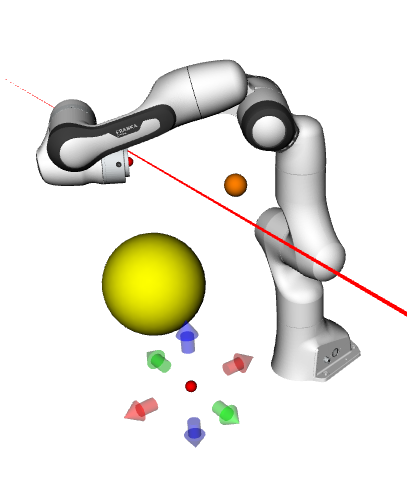
\includegraphics[width=0.45\columnwidth]{baseLine_Fail}
	\caption{Robot configuration when reactive WBQP controller (baseline approach) fails to find a solution.}
	\label{fig:robot fail}
\end{figure}

\section{Experimental Results}\label{sec-chap5:experiments}
Our goal is to highlight the main drawback of reactive WBQP discussed in the conclusions of \cref{chap:adaptive gains} and \cref{chap:robust qp}: the non-handling of potential conflict between constraints which may lead to infeasibility. In particular, the distance constraint formulated as ECBF assumes that $\confDDot\inR^n$, namely infinite deceleration capabilities, whereas $\confDDot$  often belongs to a subset  $U\subset\mathbb{R}^n$ constituted by the joint acceleration limits, torque bounds as well as other constraints. Conversely, the MPC allows solving this potential conflict by accounting for these constraints along the preview horizon and shaping the optimal targets $\command$ that fulfill those constraints.  %Unfortunately, the size of the command vector increases (and correspondingly the matrices $\Bd$ and $\stackBd$) which leads to high the MPC computation time. %as shown in~\eqref{eq:task&joint space QP with constraints} which results $\confDDot\in U\subset \mathbb{R}^n$ This situation is particularly appealing when $\confDDot\in U$ where $U$ is only a subset of $\mathbb{R}^n$. 

To validate our approach, we run simulations on the robotic arm Panda. The MPC \cref{eq:compact MPC} is implemented using COPRA library\footnote{\url{https://github.com/jrl-umi3218/copra}}. The current c++ implementation allows running the MPC in a separate thread. 
%The latter will then generate optimal targets $\eepositionOpt, \confOpt$. 
We have chosen to formulate the WBQP as in \cref{eq:task&joint space QP with constraints} to ensure dynamic consistency while tracking the MPC output. %Rather than considering the unconstrained QP~\cref{eq:task&joint space QP without constraints}, we have chosen to formulate the constrained QP~\cref{eq:task&joint space QP with constraints} in order to ensure dynamic consistency  while tracking $\eepositionOpt, \confOpt$ by the end-effector and posture tasks such that
More importantly, we consider the case where the end-effector has to avoid collision with a ball in its workspace. Let us denote $\bm{p}_{\rm ball}\inR^3$ the coordinates of the center of the ball and $r>0$ its radius. The distance between the end-effector and the ball surface is then 
\begin{equation}
	\delta(\conf) = \bm{n}_{\bm{\delta}}\tp\left(\eeposition - \bm{p}_{\rm ball}\right) - r \inR
\end{equation}
 with $\bm{n}_{\bm{\delta}}=\frac{\eeposition - \bm{p}_{\rm ball}}{||{\eeposition - \bm{p}_{\rm ball}}||}\inR^3$ is a unit vector. Consequently, to avoid the collision, the distance $h_{\rm coll}$ in \cref{eq:distance constraint forward kinematics} must fulfill
 \begin{equation}\label{eq:distance to collision constraint MPC}
 	h_{\rm coll}=\delta(\conf) - \delta_{\min} \geq0 
 \end{equation}
Then, $\dot{h}$ and $\ddot{h}$ are defined as in \cref{eq:distance constraint forward vel,eq:distance constraint forward acc} where $\mathbf{J}^{h_{\rm coll}}=\bm{n}_{\bm{\delta}}\tp\eeJac$ and $\mathbf{\dot{J}}^{h_{\rm coll}}=\bm{n}_{\bm{\delta}}\tp\eeJac + \bm{n}\tp\eeJacDot$. To make the problem more appealing, another constraint is defined for the robot CoM $\bm{CoM}(\conf)\inR^3$ to be upper bounded along the $X$-axis. This is achieved by keeping the distance $h_{\rm com}$ positive
\begin{equation}\label{eq:com constraint along X-MPC}
	h_{\rm com} = \bm{n}_{\rm com}\tp \bm{CoM}(\conf) + {CoM}_{X_{\max}} >0
\end{equation}
where $\bm{n}_{\rm com}\tp = \begin{bmatrix}
	-1 &0 &0
\end{bmatrix}\inR^3$ is a normal vector and ${CoM}_{X_{\max}}=0.2$~cm. The CoM constraint Jacobian $\mathbf{J}^{h_{\rm com}}=\bm{n}_{\rm com}\tp\mathbf{J}^{{\rm com}}\inR^{1\times n}$ and $\mathbf{\dot{J}}^{h_{\rm com}}=\bm{n}_{\rm com}\tp\mathbf{\dot{J}}^{{\rm com}}\inR^{1\times n}$ with $\mathbf{J}^{{\rm com}}\inR^{3\times n}$ the CoM Jacobian.
By constraining the CoM in \cref{eq:com constraint along X-MPC}, the robot is less free to stretch the arm to skirt the ball, and thereby it demands more complex motion for the robot to fulfill both constraints while taking into account the hardware limitations.   
 

The experiment scenario consists in generating random reference Cartesian targets $\REF{\eeposition}\inR^{m}$ ($\REF{\eevelocity}=\REF{\eeacceleration}=\zeros)$ that are forwarded to MPC\footnote{$\REF{\conf}\inR^{n}$ ($\REF{\confDot}=\REF{\confDDot}=\zeros$) is also forwarded to MPC and denotes a given reference posture with an elbow-up configuration.}. These random targets aim to lead the end-effector into a collision with the ball and the CoM to reach its maximum boundary (\cref{fig:pannda&yellowball&CoM}).
The meta-parameters of MPC and WBQP used in the experiment are shown in \cref{tab:MPC-QP parameters}.
\begin{figure}
	\centering
	\subfloat[]{
		\includegraphics[width=0.49\columnwidth]{hcoll_mpc2}
		\label{subfig:hcoll and hdotcoll MPC}}
	%	\hfil
	\subfloat[]{
		\includegraphics[width=0.49\columnwidth]{hcom_mpc2}
		\label{subfig:hcom and hdotcom MPC}}
	\caption{Time evolution of $h_{*}$ (blue) and $\dot{h}_{*}$ (orange) in the case of closed-loop MPC-WBQP control scheme:~\subref{subfig:hcoll and hdotcoll MPC} $h_{\rm coll}$ and $\dot{h}_{\rm coll}$,~\subref{subfig:hcom and hdotcom MPC} $h_{\rm com}$ and $\dot{h}_{\rm com}$. The colored bands correspond to the current assigned $\REF{\eeposition}$.}
	\label{fig:hcoll and hcom MPC}
\end{figure}
\begin{figure}
	\centering
	\subfloat[]{
		\includegraphics[width=0.49\columnwidth]{hcoll_prediction}
		\label{subfig:hcoll prediction MPC}}
	%	\hfil
	\subfloat[]{
		\includegraphics[width=0.49\columnwidth]{hcom_prediction}
		\label{subfig:hcom prediction MPC}}
	\caption{Time evolution of $h_{*}$ (blue solid) and the its predictions (colored dotted-solid) along different preview horizon in the case of closed-loop MPC-WBQP control scheme for $t\in\left[0.7,3\right]$~s (first colored band in \cref{fig:hcoll and hcom MPC}).~\subref{subfig:hcoll prediction MPC} $h_{\rm coll}$.~\subref{subfig:hcom prediction MPC} $h_{\rm com}$.}
	\label{fig:hcoll and hcom  prediction MPC}
\end{figure}
\begin{figure}
	\centering
	\subfloat[]{
		\includegraphics[width=0.33\columnwidth]{X_mpc2}
		\label{subfig:X}}
%	\hfil
	\subfloat[]{
		\includegraphics[width=0.33\columnwidth]{Y_mpc2}
		\label{subfig:Y}}
%	\hfil
	\subfloat[]{
		\includegraphics[width=0.33\columnwidth]{Z_mpc2}
		\label{subfig:Z}}
	\caption{Reference Cartesian target $\REF{\eeposition}$ (dashed blue), optimal Cartesian target $\eepositionOpt$ (orange) and end-effector position $\eeposition$ (blue).~\subref{subfig:X} X coordinate.~\subref{subfig:Y} Y coordinate.~\subref{subfig:Z} Z coordinate.}
	\label{fig:optimal target MPC}	
\end{figure}
\begin{figure}
	\centering
	\subfloat[]{
		\includegraphics[width=0.33\columnwidth]{endEff_X_prediction}
		\label{subfig:X prediction}}
	%	\hfil
	\subfloat[]{
		\includegraphics[width=0.33\columnwidth]{endEff_Y_prediction}
		\label{subfig:Y prediction}}
	%	\hfil
	\subfloat[]{
		\includegraphics[width=0.33\columnwidth]{endEff_Z_prediction}
		\label{subfig:Z prediction}}
	\caption{End-effector position $\eeposition$ (blue solid) and its predictions (colored dotted-solid) along different preview horizon in the case of closed-loop MPC-WBQP control scheme for $t\in\left[0.7,3\right]$~s (first colored band in \cref{fig:optimal target MPC}).~\subref{subfig:X} X coordinate.~\subref{subfig:Y} Y coordinate.~\subref{subfig:Z} Z coordinate.}
	\label{fig:endEff prediction MPC}	
\end{figure}
\subsection{Baseline Approach}
For comparison, we choose the baseline approach to be the reactive WBQP closed-loop control scheme shown in \cref{fig:MPC-QP}\subref{subfig:MPC-QP kinematic-controlled robot} without the MPC outer  loop.  WBQP is formulated as in~\cref{eq:task&joint space QP with constraints} to which we insert on-the-fly the collision and CoM constraints \cref{eq:collision constraint} and \cref{eq:com constraint along X-MPC} formulated as shown in \cref{eq:second order ODI distance}
\begin{align}
\label{eq:collision constraint formulated ODI}	\mathbf{J}^{h_{\rm coll}}\confDDot + \mathbf{\dot{J}}^{h_{\rm coll}}\confDot  +K_{\rm d}^{h_{\rm coll}}\dot{h}_{\rm coll} +K_{\rm s}^{h_{\rm coll}}h_{\rm coll} &\geq0, \ \text{if~} h_{\rm coll}\leq10~\text{cm},\\
\label{eq:com constraint formulated ODI}	\mathbf{J}^{h_{\rm com}}\confDDot + \mathbf{\dot{J}}^{h_{\rm com}}\confDot  +K_{\rm d}^{h_{\rm com}}\dot{h}_{\rm com} +K_{\rm s}^{h_{\rm com}}h_{\rm com} &\geq0, \ \text{if~} h_{\rm com}\leq3~\text{cm},
\end{align}
 where the constraints gains are computed as in \cref{eq:adaptive gain equation}. The results are shown in \cref{fig:hcoll and hcom time evolution-QP baseline}. \cref{fig:hcoll and hcom time evolution-QP baseline}\subref{subfig:hcoll} and \cref{fig:hcoll and hcom time evolution-QP baseline}\subref{subfig:hcom} show that when the collision and com constraints~\cref{eq:collision constraint formulated ODI} and \cref{eq:com constraint formulated ODI}, respectively, are inserted  with low initial velocities $\dot{h}_{\rm coll}$ and $\dot{h}_{\rm com}$ then the joint deceleration needed is feasible and WBQP finds a solution $\confDDot$ within the hardware limits. In this case, the collision and com constraints are compatible with the hardware limits. However, when the initial velocity is high ($\dot{h}_{\rm coll}=-1.2$~m/s shown with a thick circle), then the necessary joint deceleration to stop at the boundary is not compatible with the hardware limits, and thereby the WBQP fails to find a solution (\cref{fig:robot fail}).  


\begin{figure}
	\centering
	\includegraphics[width=0.6\columnwidth]{qRef_mpc}
	\caption{Reference posture target $\confOpt$ computed by MPC and tracked by the WBQP posture task \cref{eq:optimal posture target for QP}.}
	\label{fig:optimal posture target MPC}
\end{figure}
\begin{figure}
	\centering
	\includegraphics[width=0.32\columnwidth]{5_mpc2}
	\includegraphics[width=0.32\columnwidth]{7_mpc2}
	\includegraphics[width=0.32\columnwidth]{4_mpc2} \\
	\includegraphics[width=0.32\columnwidth]{2_mpc2}
	\includegraphics[width=0.32\columnwidth]{3_mpc2}
	\includegraphics[width=0.32\columnwidth]{6_mpc2} 
%	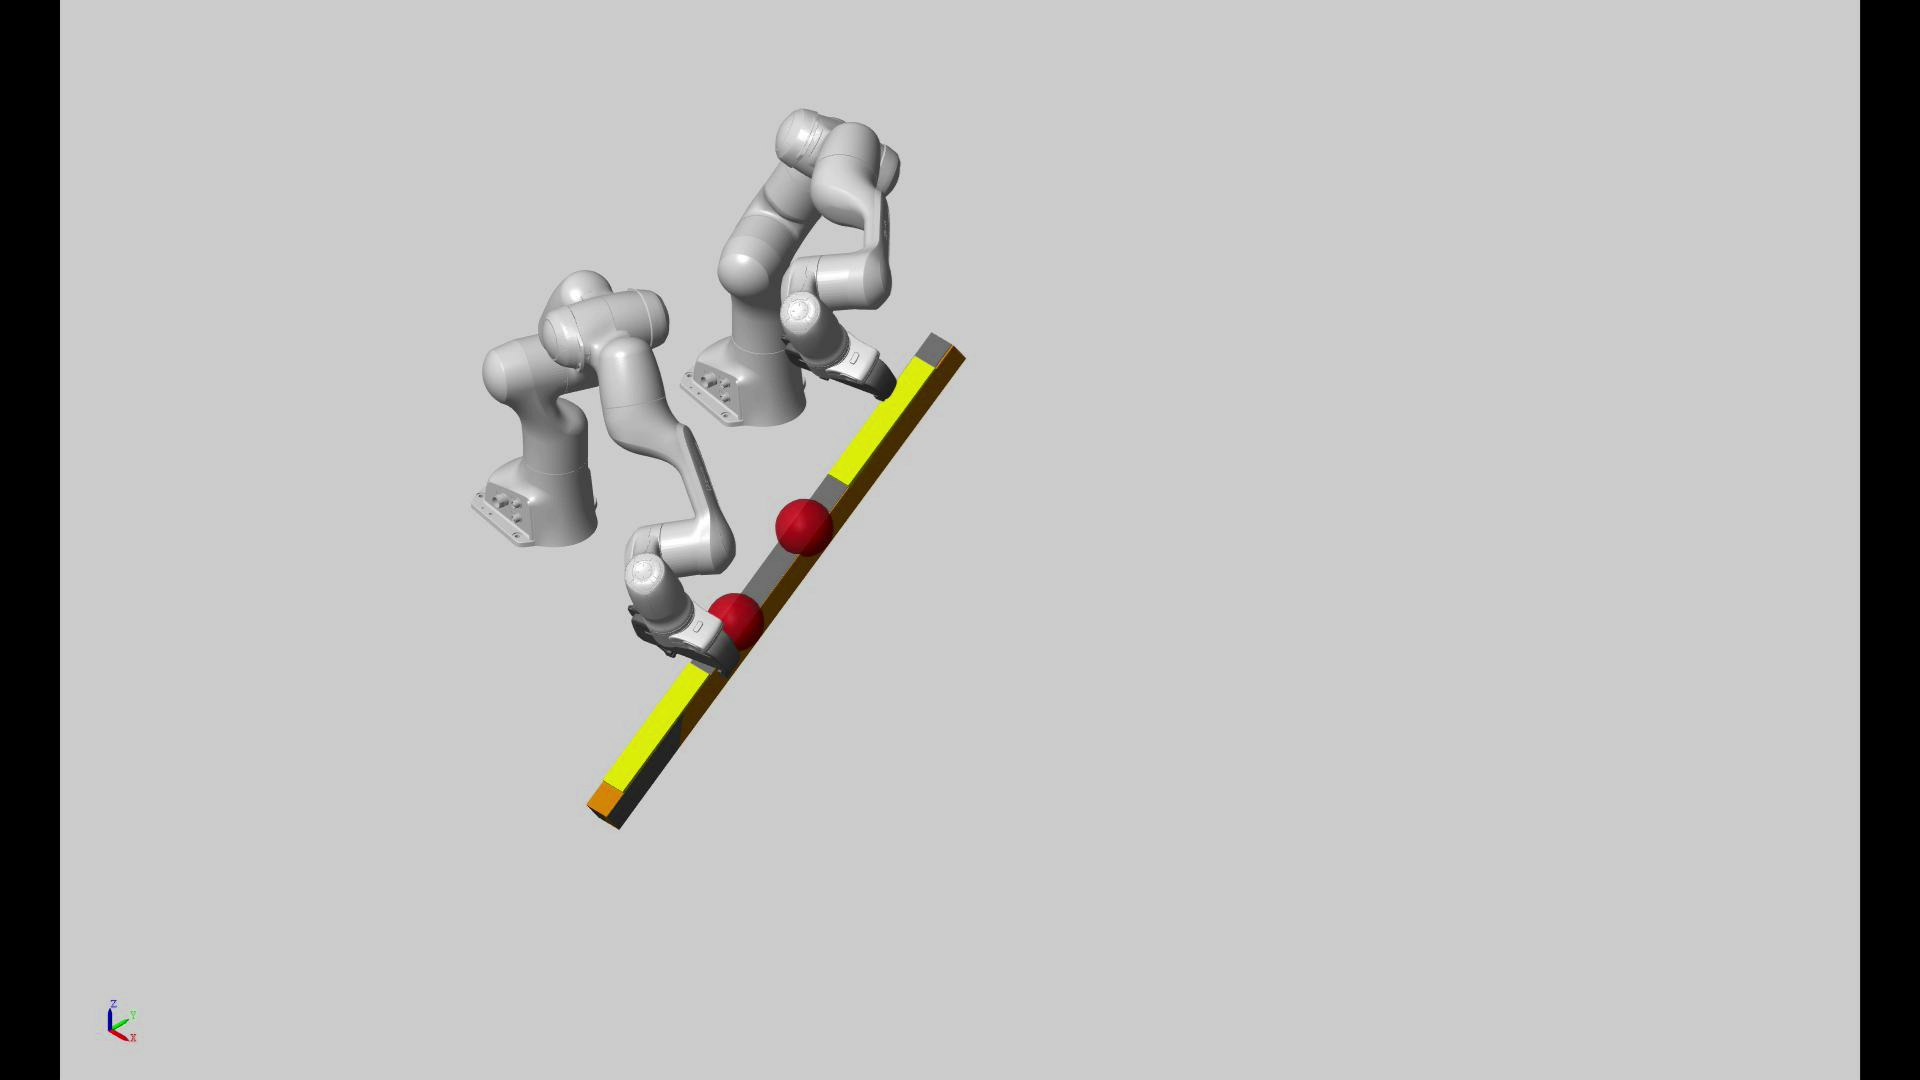
\includegraphics[width=0.25\columnwidth]{4.png}
%	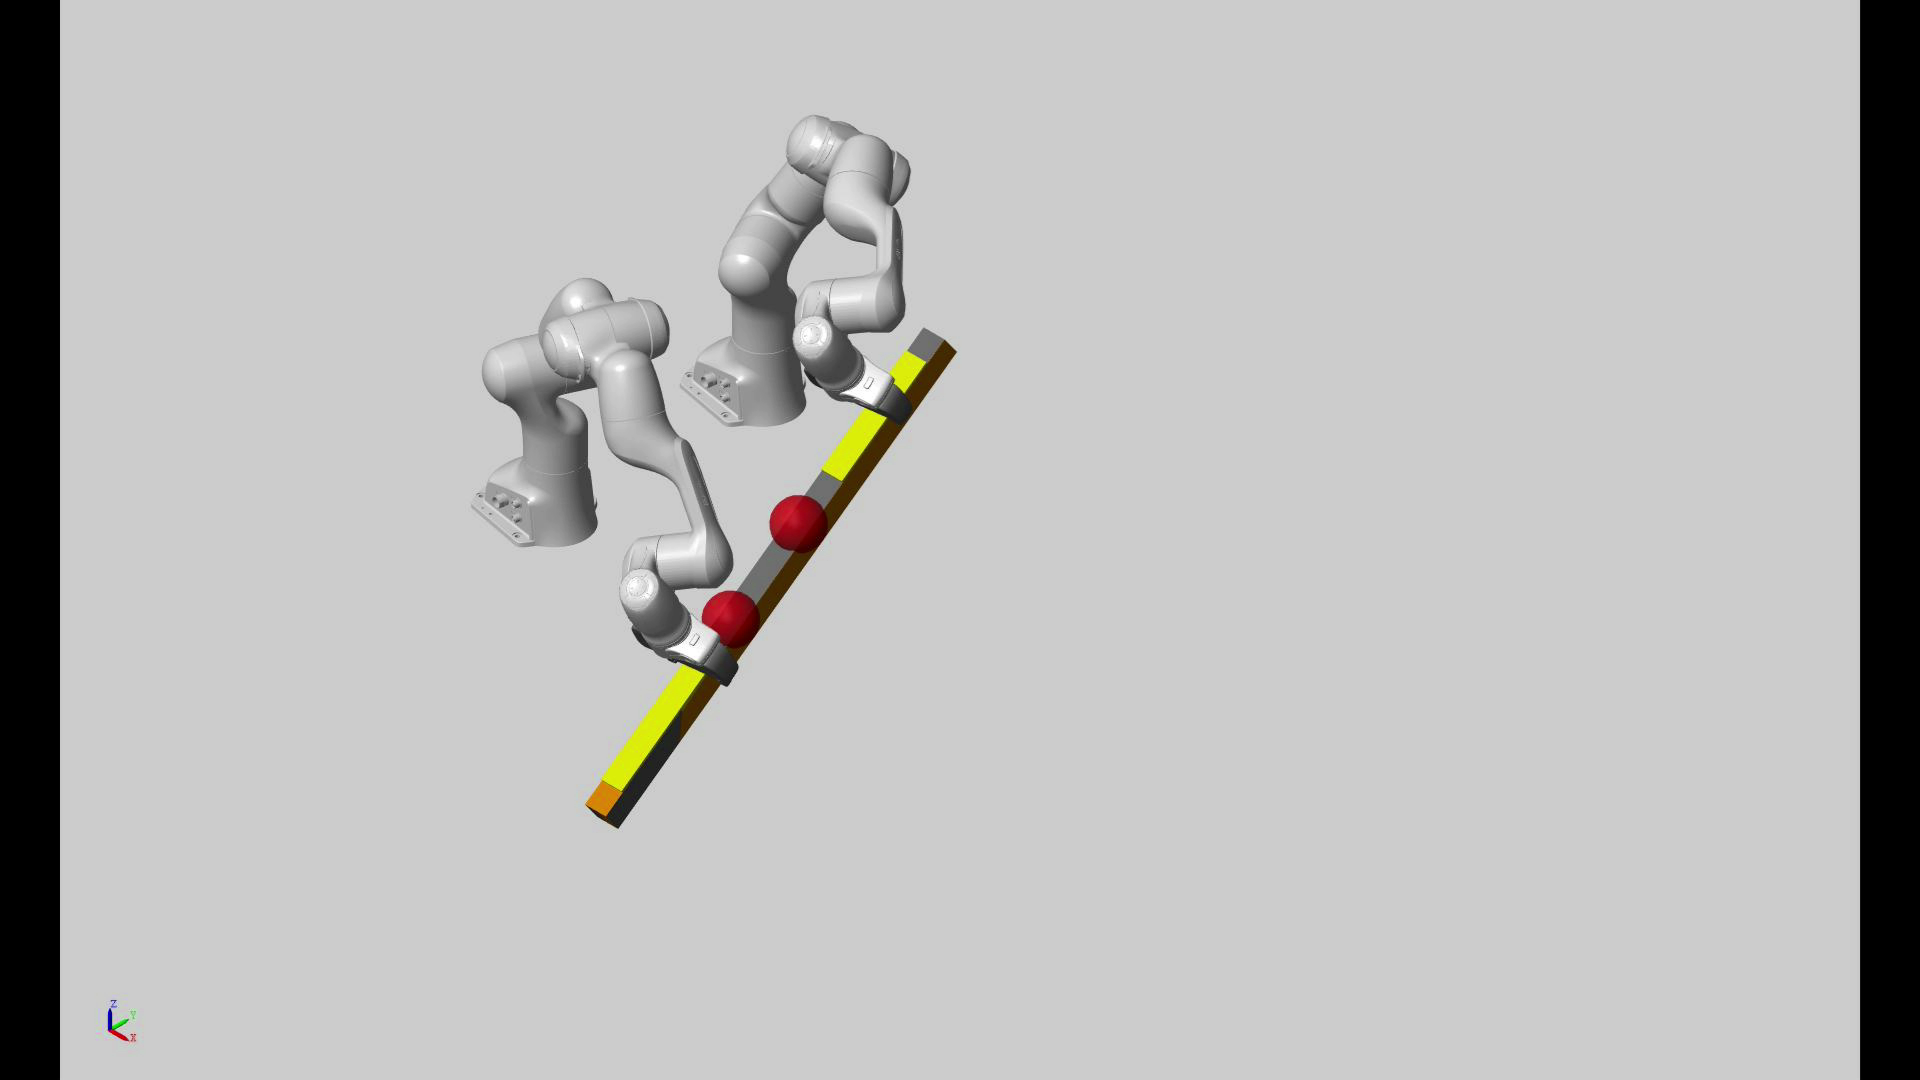
\includegraphics[width=0.2\columnwidth]{5.png}
\caption{Different screenshots of the closed-loop MPC-WBQP resulting motion. The shadowed Pandas are the robot states prediction along the preview horizon. The blue trajectory denotes the predicted end-effector $\eeposition$ position, and the predicted optimal Cartesian targets $\eepositionOpt$ are shown with graduated-green points.}
\label{fig:MPC-QP motion}
\end{figure}
\begin{figure}
	\centering
	\subfloat[]{
		\includegraphics[width=0.49\columnwidth]{hcoll_hcom_zoom_mpc2}
		\label{subfig:hcoll hcom zoomed}
	}
	\subfloat[]{
		\includegraphics[width=0.5\columnwidth]{slackness_mpc2}
		\label{subfig:slackness}
	}
	\caption{Zoom-in of $h_{*}$ near the boundary $h_{*}=0$ (dashed red) and the corresponding slackness.~\subref{subfig:hcoll hcom zoomed} $h_{\rm coll}$ (blue) and $h_{\rm com}$ (orange).~\subref{subfig:slackness} Slackness of the constraint \cref{eq:collision constraint MPC} (blue, left ordinate axis) and \cref{eq:com constraint MPC} (orange, right ordinate axis).}
	\label{fig:hcoll and hcom MPC zoomed + slackness}
\end{figure}
\begin{figure}
	\centering
	\includegraphics[width=0.6\columnwidth]{mpc_durationZ}
	\caption{MPC computation time (blue), the mean (red) and the standard deviation (dashed-yellow). The mean is $11.09$~ms with a standard-deviation of $1.22$~ms.}
	\label{fig:mpc duration}
\end{figure}
%\begin{figure}
%	\centering
%	\includegraphics[width=0.75\columnwidth]{slackness_mpc}
%	\caption{Slackness of the constraint \cref{eq:collision constraint MPC} (blue, left ordinate axis) and \cref{eq:com constraint MPC} (orange, right ordinate axis). }
%	\label{fig:slackness MPC}
%\end{figure}
\subsection{Closed-loop MPC-WBQP}
 For the MPC implementation, the state and command vectors are
\begin{equation}\label{eq:state and command for MPC-experiment}
	\state= \begin{bmatrix}
		\eeposition \\ \eevelocity \\ \conf \\ \confDot \\ h_{\rm coll} \\ \dot{h}_{\rm coll} \\ h_{\rm com} \\ \dot{h}_{\rm com} 
	\end{bmatrix}\inR^{2m+2n+4=24}, \ \command = \begin{bmatrix}
		\bm{\delta} \\ \eepositionOpt \\ \confOpt
	\end{bmatrix}\inR^{d+m+n = 19}.
\end{equation}

The matrices $\mathbf{A}_c$ and $\mathbf{B}_c$ of the dynamic model in \cref{eq:continuous-time DS} are adapted to $\state$ and $\command$ vectors in \cref{eq:state and command for MPC-experiment}. In particular, $\ddot{h}_{\rm coll}$ and $\ddot{h}_{\rm com}$ are computed as in \cref{eq:distance constraint forward acc}, and the constraints \cref{eq:distance to collision constraint MPC} and \cref{eq:com constraint along X-MPC} are formulated as in \cref{eq:MPC distance constraint}.
The collision and CoM constraint are formulated as shown in \cref{eq:MPC distance constraint}
\begin{align}
\label{eq:collision constraint MPC}	\dot{h}_{{\rm coll}_i} + \alpha h_{{\rm coll}_i}  &\geq 0 \\
\label{eq:com constraint MPC}	\dot{h}_{{\rm com}_i} + \alpha h_{{\rm com}_i}  &\geq 0
\end{align}
The slack variables relax joint position constraint \cref{eq:MPC joint-pos constraint}, joint velocity constraint \cref{eq:MPC joint-vel constraint}, and collision and CoM constraints \cref{eq:collision constraint MPC} and \cref{eq:com constraint MPC}, respectively, which makes the slack variables dimension $d=n+2=9$.

 WBQP is formulated as in \cref{eq:task&joint space QP with constraints} without considering the collision and CoM constraints formulated as ODI in \cref{eq:collision constraint formulated ODI} and \cref{eq:com constraint formulated ODI}, respectively. 
Note that we could add the collision constraint and CoM constraints formulated as second-order ODI as shown in \cref{chap:adaptive gains} to WBQP as a supplementary safety layer. However, we chose to ignore them in WBQP to explicitly show the effect of the MPC-based reference governor on constraints satisfaction. 
 
 The discretization time step is taken $\deltaT = 0.12$~s with $N=10$ steps ($T_{\rm preview}=1.2$~s).
\subsubsection{MPC Optimal Outputs Evolution}
The time evolution of $h_{\rm coll}$, $\dot{h}_{\rm coll}$, $h_{\rm com}$ and $\dot{h}_{\rm com}$ is shown in \cref{fig:hcoll and hcom MPC}. $h_{\rm coll}$ and $h_{\rm com}$ reach smoothly their boundaries with zeros velocity. Comparatively, to the baseline approach in \cref{fig:hcoll and hcom MPC}, $\dot{h}_{\rm coll}$ and $\dot{h}_{\rm com}$ are not allowed to grow excessively because the deceleration starts earlier. This effect is illustrated in   \cref{fig:hcoll and hcom  prediction MPC} which shows the current $h_{\rm coll}$ and $h_{\rm com}$ with their predictions along different preview horizon. $h_{\rm coll}$ and $h_{\rm com}$ predictions either converge smoothly  toward the boundary  or stop before it. 
More concretely, the MPC output optimal targets $\eepositionOpt$  and $\confOpt$ that account for the hardware limitations, the collision and CoM constraints, and enforces them along the preview horizon. \cref{fig:optimal target MPC} shows how the MPC  computes $\eepositionOpt$ a pathway tracked by WBQP end-effector task \cref{eq:optimal Cartesian target for QP} and which deviates from $\REF{\eeposition}$ if the constraints require that (see colored bands in \cref{fig:hcoll and hcom MPC} and \cref{fig:optimal target MPC}). An example of $\eeposition$ predictions is shown in \cref{fig:endEff prediction MPC}. Correspondingly to \cref{fig:hcoll and hcom  prediction MPC},  $\eeposition$ predictions tend be constant after $t=1.5$~s stop the end-effector motion as $h_{\rm coll}$ and $h_{\rm com}$ are close to the their boundary.
In addition, the optimal posture target $\confOpt$ in \cref{fig:optimal posture target MPC} is varying as well to fulfill the constraints. From this perspective, the WBQP posture task \cref{eq:optimal posture target for QP} is no longer a regularization task intended mainly to solve the remaining redundancies but also contributes (correspondingly to its weight $\weight_{\confDDot}$) to prevent collisions or hardware limits violation. Screenshots of the closed-loop MPC-WBQP resulting motion with the predicted states are shown in \cref{fig:MPC-QP motion}.

% The posture task is no longer a regularization task intended mainly to solve the remaining redundancies, it brings an interesting behavior for the reactive whole-body QP.

\subsubsection{Constraints Fulfillment}
Since the WBQP does not account for the collision and CoM constraints, it is important to analyze how well delegating constraints fulfillment to MPC is performing. This is even more crucial since \cref{eq:collision constraint MPC} and \cref{eq:collision constraint MPC} are handled as soft constraints. %\cref{fig:hcoll and hcom MPC zoomed} shows a zoom-in of $h_{\rm coll}$ and $h_{\rm com}$ time evolution near the boundary $h_{*}=0$. 
We can see from \cref{fig:hcoll and hcom MPC zoomed + slackness}\subref{subfig:hcoll hcom zoomed} that $h_{\rm coll}$ and $h_{\rm com}$ slightly overshoot the boundary $h_{*}=0$ ($\leq 5\cdot10^{-5}$~m) before converging back to the boundary thanks to the asymptotic convergence property ensured by the constraint formulation \cref{eq:com constraint MPC} and \cref{eq:collision constraint MPC}. This slight violation is due to three factors:  the slack variables, the non-modeled joint dynamics since the experiment is performed with a kinematic-controlled robot as already discussed in \cref{chap:robust qp}, and the low MPC running frequency comparatively to the WBQP (namely the constraint can be violated within one MPC computation iteration).
%Nevertheless, it seems to be highly due the second factor rather than the first one. 
\cref{fig:hcoll and hcom MPC zoomed + slackness}\subref{subfig:slackness} shows non-zero slackness of both constraints \cref{eq:collision constraint MPC} and \cref{eq:com constraint MPC}.  Interestingly, relaxing these constraints does not systematically imply their violation. In fact, $h_{\rm coll}$ is strictly positive for $t\in\left[27.5,40\right]$~s, yet the corresponding slack variable is continuously non-null. We argue that this is because all the constraints are permanently introduced in MPC QP. Hence, the kinematic constraints can be active even when they are far from their boundaries and be potentially relaxed.
%the slackness is in terms of velocity and not in terms of distance: relaxing the velocity is less critical in the long run than relaxing the distance. 
The slack variables relative to the $\confDot$ constraints are not plotted because they are null (i.e., joint-position and velocity bounds enforced as hard constraints).
\subsubsection{Computation Time and Prediction Accuracy} 
Let us now analyze the prediction accuracy of our MPC-WBQP control scheme. We recall that we assume that the Jacobians and EoM matrices and vectors remain constant along the preview horizon to have a linear model for the MPC. From \cref{fig:hcoll and hcom  prediction MPC} and \cref{fig:endEff prediction MPC}, we can see that each current state matches accurately the prediction during at least 3 epochs (i.e., during $3\times 120 = 360$~ms). Beyond that, the prediction accuracy decreases since the conservatism effect may be more predominant\footnote{The highest prediction error is observed in \cref{fig:endEff prediction MPC}\subref{subfig:Z prediction} which is only $5$~cm at the end of the preview horizon $T_{\rm preview}=1.20$~s.}. This accuracy is due to the relatively low MPC computation time shown in \cref{fig:mpc duration} which allows refreshing the MPC computation at an average frequency of $90.21$~Hz. The computation time depends mainly on the size of $\stackCommand$ which is related to the number of prediction steps $N$ and the size of the command vector $\command$. In particular, in our simulation, $\stackCommand\inR^{209}$. Hence, improving the computation time boils down to either reducing $\command$ vector size or decreasing the length of the preview horizon. The first option is tricky as $\command$ size depends mostly on the robot DoF number and tasks dimension to be controlled. Another possibility is to lower the dimension of the slack variables $d$  by rendering some constraints hard, which may endanger the MPC feasibility. On the other hand, the second option alters the prediction abilities and approaches the myopic WBQP. Balancing between the prediction capabilities, MPC feasibility, and the computation time is a well-known dilemma that generally depends on the robot, the application, and the case-study.    


%In task-space, the deceleration is due to the deviation of the optimal target $\eepositionOpt$ from $\REF{\eeposition}$ if the latter leads $h_{\rm coll}$ and/or $h_{\rm com}$ to reach their boundaries. Thanks the preview horizon, the MPC predicts the future states and enforces the hardware limitations, and the collision and CoM constraints along the preview horizon. As shown in \cref{fig:optimal target MPC},  % the collision constraint and/or the  the predicted $h_{\rm coll}$ and $h_{\rm com}$ are approaching the zero boundary. 
%This de Since the hardware limitations are enforced as hard constraints, the dece lead the robot into collision. computed by MPC that the consequence of translated into a deviat 

%TODO: the velocity $\dot{h}_{\rm coll}$ is not allowed to grow excessively which is interpreted as the deceleration is performed earlier



%Results points:
%\begin{itemize}
%%	\item $h_{\rm coll}$ and $h_{\rm com}$ time evolution with MPC-QP approach
%%	\item $\REF{\eeposition},\eepositionOpt, \eeposition$ time evolution
%%	\item Slack variables relative to  $h_{\rm coll}$ and $h_{\rm com}$ constraints
%%	\item Screenshots of the robot with MPC
%%	\item Plot of predictions 
%%	\item Modify the formulation of the constraint relative to q: CBF (asymptotic stability and forward invariance) + optimized slack variables=
%%	\item MPC and QP computation time w.r.t $N$ 
%\end{itemize}

%\begin{itemize}
%	\item Why QP-based MPC: to account explicitly for constraints 
%	\item Compare with~\cite{grandia2021icra}, more importantly\cite{zeng2021acc2}. General citation~\cite{kleff2021icra,minniti2022ral} also \cite{bemporad1998tac} for the argumentation
%	\item See feasibility explanation in~\cite{zeng2021acc1,zeng2021acc2} 
%%	\item How to initialize the initial state $\state_{0}$
%%	\item The current c++ implementation allows choosing whether or not to run the MPC in a separate thread!
%%	\item The MPC implementation is performed using the COPRA library
%%	\item The choice of $N$ and $\deltaT$.
%%	\item Targets maybe outside the robot workspace. 
%%	\item The motion dynamics is tuned using the MPC cost-function weights rather than Whole-body QP task gains.
%%	\item The resulting motion is complex: the robot does not move in a straight-line like motion. 
%%	\item The MPC runs in a separate thread at a low frequency such that it launches a new computation right after finishing the previous one. In simulation the MPC runs at approximately $40$~Hz. \textbf{When we reduce the slack variable dimension to $d=9$ instead of $d=16$ by reformulating the joint-position constraint formulation in terms of velocity, the MPC computation time drops from $25$~ms to $10$~ms which enables the MPC to run at approximately $100$~Hz.}
%%	\item MPC Feasibility is ensured by means of slack variables. Relaxing the constraints is mainly to ensure that MPC feasibility if $\state_{0}$ violates the constraints due to non-modeled dynamics, noise or communication delays.  Yet, this is still better than using QP with relaxed constraints since it only guarantees point-wise feasibility without any preview of the future states~\cite{zeng2021acc1}.
%\end{itemize}
\section{Conclusion}\label{sec-chap5:conclusion}
In this chapter, we proposed a solution for constraints incompatibility, a well-known issue of multi-objective QP-based control approaches. To handle the potential conflict between constraints, our method consists of implementing an MPC-based reference governor which encapsulates the inner loop constituted by the WBQP controller and the robot. Based on the closed-loop dynamics of the tasks and constraints,  MPC outputs tasks' optimal targets to be tracked by multi-objective WBQP such that the hardware limits and safety constraints are enforced forward in time along the preview horizon. In particular, we showed that the optimal end-effector Cartesian targets avoid collision with an obstacle and keep the robot CoM bounded without even considering these constraints in the WBQP controller.
The proposed closed-loop MPC-WBQP control scheme outperforms the purely reactive (myopic) WBQP, where the constraints introduced online may lead to an empty feasibility domain. 

Despite the conservativeness of our method to keep the MPC model linear, we showed that the state's prediction accuracy justifies the soundness of our assumptions. 
In this context, future works will be conducted to enhance the MPC with a Jacobians prediction scheme that will considerably lower the conservativeness and improve the prediction precision. Hierarchical architecture proposed in~\cite{li2021ral} can also be a good compromise between prediction accuracy and computation simplicity. Moreover, experiments on Panda robot shall be performed.
%lower this conservatism by considering prediction models for the Jacobians and EoM matrices which enables to have a more accurate prediction. 
Also, establishing/breaking/maintaining contacts while moving~\cite{romualdi2022icra} is an interesting continuation topic of the presented work. 

In addition, we so far considered only tasks whose errors evolve in a Euclidean space. Typically, the orientation task error evolves in a non-Euclidean manifold, preventing straightforwardly including them into the current MPC linear implementation. Research work is currently conducted in this direction based on predicting the orientation of the local tangent space to exploit its Euclidean properties. 
Furthermore, theoretical studies need to be performed to analyze the closed-loop MPC-WBQP stability with sufficient conditions on the existence of solutions.

The next chapter introduces a strategy to unify observation and control. This strategy is based on a new idea of \emph{tasks-interdependency} in the context of multi-objective QP control. Namely, we intend to formulate a task whose reference is the output of another task. This new concept of multi-objective QP control framework allows us to combine tasks that may be \emph{coupled}: \emph{estimation} and \emph{tracking}, for instance. We then show how this new idea is judiciously exploited to formulate human-robot handover control. 
%the MPC model is based on the closed-loop dynamics of the tasks and constraints of interests and which is obtained by the closed-form solution an unconstrained weight-prioritized QP. 
%Thanks to its preview horizon, the MPC acts then as a constraints manager by outputting task optimal targets which fulfill the constraints. 
%TODO: - the appraoch outperforms the purely reactive (myopic) QP where the constraints introduced online may lead to an empty constraint set and thereby to QP infeasiblity. The results shows promising results despite the rough approximation made to keep the MPC linear.
%TODO:- see Niels email for constraints managing.   
%$$
%\weight_1^2 \norm{\qjacobian \qaccelerations  - \left( \PD{\eeacceleration} - \qjacobianDot \CUR{\qvelocities} \right)} 
%$$
%whereas the second objective aims to track PD joint accelerations \eqref{eq::jointspacePD} with weight $\weight_2^2>0$
%$$
%\weight_2^2 \norm{\identityMatrix \qaccelerations - \PD{\qaccelerations}}$$




%Combining the two weighted objectives \eqref{eq::taskspacePD} and \eqref{eq::jointspacePD},
%the classical quadratic problem~(QP) representing the whole-body controller writes
%\begin{IEEEeqnarray}{rCl}
%	\label{eq::mainQP}
%	\CUR{\qaccelerations}
%	= & \argmin_{ \qaccelerations } \hspace{0.2cm} & %todo \frac{1}{2} 
%	\norm{
%		\begin{bmatrix}
%			\weight_1 \qjacobian \\
%			\weight_2 \, \identityMatrix
%		\end{bmatrix}
%		\qaccelerations -
%		\begin{bmatrix}
%			\weight_1 \left( \PD{\eeacceleration} - \qjacobianDot \CUR{\qvelocities} \right) \\
%			\weight_2 \PD{\qaccelerations} 
%		\end{bmatrix}
%	}
%	\hspace{0.4cm}
%	%\nonumber 
%	\\ %############################################
%	& \text{s.t.} & 
%	%& \text{s. t. } &  
%	\qaccelerationsLowerBound \leq \qaccelerations \leq \qaccelerationsUpperBound
%	\nonumber 
%	\\ %############################################
%	&  & 
%	\qtorquesLowerBound - \qcoriolisMatrix \CUR{\qvelocities} - \qgravityMatrix
%	\leq \qinertia \qaccelerations 
%	\leq \qtorquesUpperBound - \qcoriolisMatrix \CUR{\qvelocities} - \qgravityMatrix
%	\nonumber
%\end{IEEEeqnarray}
%which can also be written as
%\begin{IEEEeqnarray}{rCl}
%	\label{eq::mainQP}
%	\CUR{\qaccelerations}
%	= & \argmin_{ \qaccelerations } \hspace{0.2cm} & %todo \frac{1}{2} 
%	\norm{
%		\begin{bmatrix}
%			\weight_1 \identityMatrix, & 0 \\
%			0, & \weight_2 \identityMatrix
%		\end{bmatrix}
%		\left(
%		\begin{bmatrix}
%			\qjacobian \\
%			\identityMatrix
%		\end{bmatrix}
%		\qaccelerations -
%		\begin{bmatrix}
%			\PD{\eeacceleration} - \qjacobianDot \CUR{\qvelocities} \\
%			\PD{\qaccelerations} 
%		\end{bmatrix}
%		\right)
%	}
%	\hspace{0.4cm}
%	%\nonumber 
%	\\ %############################################
%	& \text{subject to } & 
%	%& \text{s. t. } &  
%	\qaccelerationsLowerBound \leq \qaccelerations \leq \qaccelerationsUpperBound
%	\nonumber 
%	\\ %############################################
%	&  & 
%	\qtorquesLowerBound - \qcoriolisMatrix \CUR{\qvelocities} - \qgravityMatrix
%	\leq \qinertia \qaccelerations 
%	\leq \qtorquesUpperBound - \qcoriolisMatrix \CUR{\qvelocities} - \qgravityMatrix
%	\nonumber
%\end{IEEEeqnarray}